\chapter{第三章 总体架构设计}
\section{系统设计目标}
\subsection{高保真性}
高保真性是本系统的核心目标之一,要求生成的交通场景能够最大限度地忠实反映自然语言描述。为了实现这一目标,系统不仅需要保证场景的视觉效果和语义的一致性,还应考虑各种复杂的环境要素和交通行为的准确性。例如,生成的场景中各类交通工具的行为需要与现实世界中的交通流动一致,交通规则和行为模式需要严格遵循。因此,系统需要通过对输入描述进行精确解析,使用先进的自然语言处理技术(如大语言模型)来理解场景中的各种细节,并转换为对应的三维仿真环境。这些细节不仅仅是物理上的位置和对象,更包括交通元素之间的动态互动,环境条件如天气、时间、光照等因素的考虑。

\subsection{自动化}
自动化是本系统设计的另一个关键目标。通过实现从自然语言输入到场景生成与仿真运行的自动化流程,系统能够减少人工干预,提高效率并降低人为错误的发生。系统应能够通过少量的用户输入(例如一段简短的自然语言描述)完成从场景构建到仿真运行的全过程,自动生成所有必要的配置文件,调度仿真平台执行,并收集仿真结果进行后续分析。自动化不仅限于场景生成,也包括场景的评估和结果展示,能够在生成后直接对场景进行可视化、量化评估,并输出最终报告。这种全自动的流程将极大地提升仿真研究的效率,支持大规模的实验和多样化的场景生成需求。

\subsection{可扩展性}
可扩展性是系统设计中的重要原则,确保系统能够随着需求的变化进行功能和技术的扩展。系统设计应当采用模块化的结构,每个功能模块(如自然语言处理、场景生成、仿真执行、评估展示等)都可以独立发展和优化,并与其他模块无缝衔接。可扩展性体现在以下几个方面:
\begin{itemize}
	\item 自然语言处理模型的升级:随着自然语言处理技术的发展,新的语言模型和算法可能会不断出现,系统应当能够灵活集成新的语言模型,提升场景生成的准确性和多样性。
	\item 仿真平台的集成:虽然当前平台使用CARLA作为仿真引擎,未来可能会考虑集成其他仿真平台或与不同的驾驶仿真系统对接,以支持更多元的实验需求和不同平台的比较。
	\item 评估指标的多样性:系统的评估模块应支持定制化和多维度的评估指标,未来可以根据不同的场景类型、研究需求或应用场景,添加新的评估标准,改进现有评估方法。
\end{itemize}

\subsection{核心功能实现}
本系统的核心功能涵盖三个关键方面:
\begin{itemize}
	\item 从自然语言描述中自动生成三维交通场景:这一功能是系统的基础,旨在通过对输入的自然语言进行理解,自动生成能够在仿真环境中运行的交通场景。系统将利用自然语言处理模型和检索增强技术,结合已有的场景模板和元素库,实现语义精确的场景建模。
	\item 对生成的场景进行仿真与可视化:该功能主要确保生成的三维场景能够在仿真平台中正确呈现并运行。系统通过调用仿真平台API,自动将生成的场景描述转化为可执行的仿真环境,并进行实时仿真与动态可视化。此过程还包括对场景中交通元素的行为模拟,例如交通流、车辆行驶轨迹、交互等。
	\item 对生成结果进行量化评估:评估是本系统不可或缺的一部分,它提供了对生成场景质量的定量分析。系统将根据语义保真度、场景多样性和驾驶性能等指标,进行评估并生成相应的报告。通过量化评估,系统能够为场景生成提供反馈,以便后续优化,并且为自动驾驶算法的性能测试提供参考。
\end{itemize}

\subsection{系统目标的长期愿景}
随着技术的进步,系统应逐步向更高保真度、更强可扩展性、更高效自动化方向发展。在未来的版本中,系统可以集成更多的感知模型、智能决策系统等技术,进一步提升场景的复杂性与真实性。同时,系统的评估模块也可以通过引入更多的智能分析工具,提供更细粒度的结果评估,如行为预测、决策模型评估等。此外,随着自然语言处理技术的进步,系统能够处理更加复杂的语言输入和场景需求,满足更广泛的仿真测试场景需求,支撑更为丰富的自动驾驶研究与开发。

\section{系统总体架构}
系统整体架构如图3-1所示,主要分为三个核心模块:自然语言理解与场景生成模块、场景合成与仿真模块、场景评估与展示模块。数据流动过程如下:
\begin{enumerate}
	\item 用户输入自然语言指令;
	\item 系统通过检索增强与大语言模型解析自然语言,生成对应的Scenic场景描述脚本;
	\item Scenic脚本由Scenic解析器处理,并通过CARLA仿真平台进行三维场景构建与动态仿真;
	\item 仿真完成后系统采集结果数据,包括场景截图与驾驶轨迹;
	\item 对生成场景进行量化评估,输出语义保真度、多样性与驾驶性能相关指标。
\end{enumerate}
\begin{figure}[H]
	\centering
	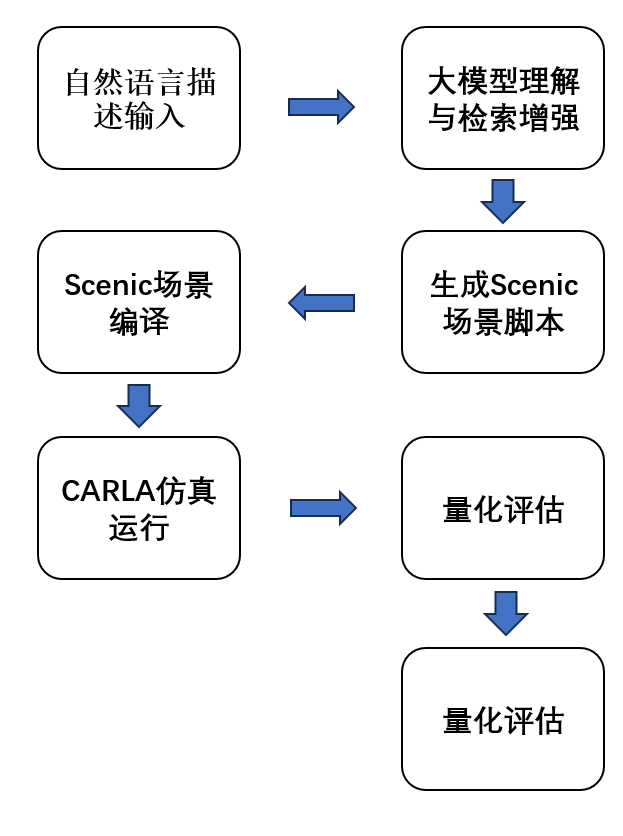
\includegraphics[width=0.9\textwidth]{../images/系统架构图.png} 
	\caption{系统架构图}
	\label{fig:system_architecture} % 添加合适的label
\end{figure}

\section{主要模块功能设计}
\subsection{自然语言理解与场景生成模块}
本模块负责接收自然语言输入并生成对应的Scenic场景描述。具体流程如下:
\begin{itemize}
	\item \textbf{输入}:自然语言形式的场景描述,例如“一个红色轿车在城市路口等待绿灯”。
	\item \textbf{检索增强}:使用 \texttt{sentence-transformers} 中的 \texttt{sentence-t5-large} 模型对输入进行向量化表示,并在本地检索数据库(如 \texttt{retrieve/scenario\_descriptions.txt})中查找相似描述作为参考样本。
	\item \textbf{大语言模型解析}:采用预训练的大语言模型(如 GPT-4o),结合检索到的参考样本,生成符合输入语义的 Scenic 脚本。
	\item \textbf{场景拼接机制}:根据场景复杂度,支持对多个子元素(如车辆、行人、环境条件)进行组织与拼接。
\end{itemize}


\subsection{场景合成与仿真模块}

本模块负责将自然语言生成的Scenic脚本转化为三维可视化仿真场景,并在CARLA仿真平台上实现动态运行。整个过程包括脚本解析、场景构建、仿真控制、交互支持与数据输出等多个环节,具体如下:

\begin{itemize}
	\item \textbf{Scenic解析}:本系统首先通过Scenic内置的语法与语义分析器对输入脚本进行解析。Scenic作为一种领域专用语言,允许用户以简洁、结构化的方式描述场景元素(如车辆、行人、障碍物等)的初始状态和约束条件。解析过程会生成包含对象属性(位置、速度、朝向)、交互规则(如跟车距离、避让行为)以及环境条件(如天气、时间)的完整场景配置。
	
	\item \textbf{仿真构建}:在完成脚本解析后,系统自动将Scenic生成的中间配置映射到CARLA仿真平台中。具体包括载入指定地图、部署交通参与者、设定传感器参数(如摄像头、LiDAR)、配置环境因素(如天气、光照、路况)等。系统可根据配置实现对城市道路、高速公路、十字路口等多种类型场景的精准建模。
	
	\item \textbf{接口调用关系}:Scenic通过其与CARLA集成的Python API调用底层仿真接口。系统自动完成Actor的创建、状态初始化、行为脚本绑定等任务,极大简化了从脚本到仿真的转换流程。研究人员无需手动编程,即可通过文本控制仿真流程,显著提高效率与复用性。
	
	\item \textbf{动态交互支持}:系统支持高度动态化场景仿真,能模拟交通参与者之间的交互行为,如车辆变道、避障、红绿灯响应、行人横穿马路等。Scenic语言提供了条件触发与时间控制机制,允许描述复杂行为序列,实现具有时序性、可演化的场景变化,增强了仿真的真实感与复杂性。
	
	\item \textbf{多样化仿真配置}:本模块支持灵活的仿真参数配置,包括地图选择(如Town01、Town05)、天气设置(晴天、雨天、雾天)、交通流量控制、车辆控制模式(自动驾驶、手动控制)等,可满足不同测试需求。同时也支持使用不同版本的CARLA和Scenic组合,具有较好的兼容性与可拓展性。
	
	\item \textbf{数据采集与输出}:在仿真执行过程中,系统可实时采集关键数据,包括传感器输出(RGB图像、深度图、点云等)、车辆状态(位置、速度、加速度)、交互事件(碰撞、刹车、偏航)等。采集数据可用于后续的模型训练、行为评估或性能对比等任务,支撑多种研究方向。
	
\end{itemize}


\subsection{场景评估与展示模块}

场景评估与展示模块旨在对生成的三维仿真场景进行可视化呈现与定量分析。该模块不仅便于研究人员直观了解场景生成效果,也为后续的性能比较、模型调优与系统验证提供了评估依据。该模块包含以下几个关键功能:

\begin{itemize}
	\item \textbf{可视化展示}:在仿真过程中,系统可自动截取关键帧截图或录制完整仿真过程视频,保存为图像或视频文件,供研究人员用于人工审阅、可视化报告展示以及用户研究评估。截图通常选择交通事件发生点(如刹车、避障、碰撞等)或特定时序节点,确保展示信息的代表性与丰富性。视频部分可通过CARLA原生录制功能或集成第三方渲染引擎实现,支持多角度、多摄像机的可视观察,进一步增强场景调试与验证的可操作性。
	
	\item \textbf{量化评估}:本系统在自动化生成与仿真的基础上,进一步引入多维度的量化评估指标,对场景生成的有效性、合理性和多样性进行定量测量,具体包括:
	
	\begin{itemize}
		\item \textbf{语义保真度(Semantic Fidelity)}:该指标用于衡量输入的自然语言描述与最终生成仿真场景之间的语义一致性。可采用人工标注评分与自动化匹配算法相结合的方式进行。例如,通过设定关键语义要素(如地点、交通行为、天气条件)匹配程度,对场景是否准确还原用户意图进行评分。自动方法可以结合自然语言处理与图结构匹配技术实现初步评估,提升效率。
		
		objectivec
		复制
		编辑
		\item \textbf{多样性指标(Scene Diversity)}:此项指标反映系统生成场景在多次输入不同自然语言后的差异性和覆盖范围。主要包括空间多样性(不同地图位置、道路类型)、元素多样性(参与车辆、行人、非机动车种类)、行为多样性(速度控制、路线选择、交通交互等)。统计方法包括使用Shannon熵、Jaccard相似度或聚类分布指标等,全面反映生成系统的泛化能力与表现范围。
		
		\item \textbf{驾驶性能指标(Driving Performance)}:为了评估生成场景对自动驾驶系统的测试价值,本模块支持在生成场景中运行预设自动驾驶控制系统(如基于CARLA的自动驾驶Agent),并记录其表现。关键评估维度包括碰撞率(单位场景中发生碰撞的比例)、任务成功率(是否成功完成任务或驶出场景)、路径偏离率(与理想路径的偏差程度)等。这些数据可用于评估生成场景的挑战性与安全测试覆盖度,是场景质量评估的重要依据。
	\end{itemize}
	
	\item \textbf{评估结果展示与导出}:系统支持将评估结果以图表、表格等形式进行可视化展示,方便研究人员进行对比分析与结果报告生成。所有截图、评估指标与分析数据可导出为标准格式文件(如CSV、JSON、PNG等),用于论文撰写、模型调试或进一步的数据挖掘。
	
\end{itemize}